\documentclass[../main/main.tex]{subfiles}

\newdate{date}{21}{09}{2020}

% \begin{figure}[h!]
% \centering
% \includegraphics[page=6,width=0.8\textwidth]{../lessons/pdf_file/01_lecture.pdf}
% \end{figure}

%\displaydate{date}. Compiled:  \today. Alice.

\begin{document}


\section{Lecture 1}


\subsubsection*{Slide 1-2}

\begin{minipage}[]{0.5\linewidth}
\centering
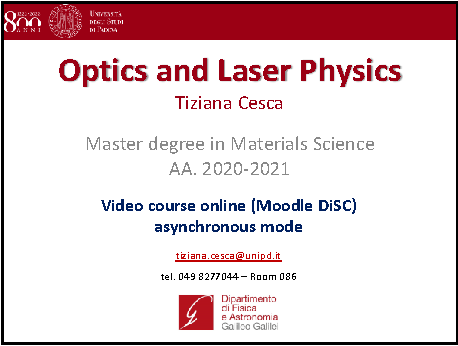
\includegraphics[page=1,width=1\textwidth]{../lessons/pdf_file/01_lecture.pdf}
\end{minipage}
\begin{minipage}[]{0.5\linewidth}
\centering
\includegraphics[page=2,width=1\textwidth]{../lessons/pdf_file/01_lecture.pdf}
\end{minipage}

\subsubsection*{Slide 3-4}

\begin{minipage}[]{0.5\linewidth}
\centering
\includegraphics[page=3,width=1\textwidth]{../lessons/pdf_file/01_lecture.pdf}
\end{minipage}
\begin{minipage}[]{0.5\linewidth}
\centering
\includegraphics[page=4,width=1\textwidth]{../lessons/pdf_file/01_lecture.pdf}
\end{minipage}

\subsubsection*{Slide 5-6}

\begin{minipage}[]{0.5\linewidth}
\centering
\includegraphics[page=5,width=1\textwidth]{../lessons/pdf_file/01_lecture.pdf}
\end{minipage}
\begin{minipage}[]{0.5\linewidth}
\centering
\includegraphics[page=6,width=1\textwidth]{../lessons/pdf_file/01_lecture.pdf}
\end{minipage}


\newpage

\subsubsection*{Slide 7}

\begin{minipage}[]{0.5\linewidth}
\centering
\includegraphics[page=7,width=1\textwidth]{../lessons/pdf_file/01_lecture.pdf}
\end{minipage}
\hspace{0.3cm}\vspace{0.3cm}
\begin{minipage}[c]{0.47\linewidth}
The field of lasers is very active also in term of research.
\end{minipage}

\subsubsection*{Slide 8}

\begin{minipage}[]{0.5\linewidth}
\centering
\includegraphics[page=8,width=1\textwidth]{../lessons/pdf_file/01_lecture.pdf}
\end{minipage}
\hspace{0.3cm}\vspace{0.3cm}
\begin{minipage}[c]{0.47\linewidth}
We will cover many different topics: from classical optics to quantum optics. The concept of classical optics will be only briefly recaped.
\end{minipage}

\subsubsection*{Slide 9}

\begin{minipage}[]{0.5\linewidth}
\centering
\includegraphics[page=9,width=1\textwidth]{../lessons/pdf_file/01_lecture.pdf}
\end{minipage}
\hspace{0.3cm}\vspace{0.3cm}
\begin{minipage}[c]{0.47\linewidth}
Here there is a list of different textbooks. Three books are highlithed, one for each topic. "Introduction to Modern Optics" is a good book for recap the concept. The exam is a written exam in which you will have an open question and you have to solve an exercise.
\end{minipage}

\subsubsection*{Slide 10}

\begin{minipage}[]{0.5\linewidth}
\centering
\includegraphics[page=10,width=1\textwidth]{../lessons/pdf_file/01_lecture.pdf}
\end{minipage}
\hspace{0.3cm}\vspace{0.3cm}
\begin{minipage}[c]{0.47\linewidth}
Light is a electromagnetic wave which can be described by the Maxwell's equations.
\end{minipage}

\subsubsection*{Slide 11}

\begin{minipage}[]{0.5\linewidth}
\centering
\includegraphics[page=11,width=1\textwidth]{../lessons/pdf_file/01_lecture.pdf}
\end{minipage}
\hspace{0.3cm}\vspace{0.3cm}
\begin{minipage}[c]{0.47\linewidth}
These are the corresponding equations when we are working in a medium. In this course, the media we are takling about are non magnetic and non conductive, hence we will talk only of \textbf{dielectric materials}. The material we are considering (used as optical elements) are typical \textbf{linear} materials, so the relation between polarization vector and electric field is linear.
\end{minipage}

\subsubsection*{Slide 12}

\begin{minipage}[]{0.5\linewidth}
\centering
\includegraphics[page=12,width=1\textwidth]{../lessons/pdf_file/01_lecture.pdf}
\end{minipage}
\hspace{0.3cm}\vspace{0.3cm}
\begin{minipage}[c]{0.47\linewidth}
It is very easy to demonstrate that applying the first equality, from the Maxwell's equation is possible to write a wave equation for both electric and magnetic fields. Hence, both electric and magnetic field are solution of a wave equation.
\end{minipage}

\subsubsection*{Slide 13}

\begin{minipage}[]{0.5\linewidth}
\centering
\includegraphics[page=13,width=1\textwidth]{../lessons/pdf_file/01_lecture.pdf}
\end{minipage}
\hspace{0.3cm}\vspace{0.3cm}
\begin{minipage}[c]{0.47\linewidth}
From the solution of the wave equation it is very easy to demonstrate that light is \textbf{transeverse} electromagnetic wave (the plane of oscillation of electric and magnetic field is transerve with respect to the propagation vector \( \va{k} \)).
An important thing is that:
\begin{equation*}
  \va{E} \times \va{B} \propto \va{k}
\end{equation*}
The amplitude of electric and magnetic field are related to phase velocity of the wave:
\begin{equation*}
  E = \frac{\omega }{k} B = c B
\end{equation*}
The phase velocity is \( c \) in vacuum.
\end{minipage}

\subsubsection*{Slide 14}

\begin{minipage}[]{0.5\linewidth}
\centering
\includegraphics[page=14,width=1\textwidth]{../lessons/pdf_file/01_lecture.pdf}
\end{minipage}
\hspace{0.3cm}\vspace{0.3cm}
\begin{minipage}[c]{0.47\linewidth}
These are the formula in a medium. The phase velocity in the medium will change with respect to the refractive index.
\end{minipage}

\subsubsection*{Slide 15}

\begin{minipage}[]{0.5\linewidth}
\centering
\includegraphics[page=15,width=1\textwidth]{../lessons/pdf_file/01_lecture.pdf}
\end{minipage}
\hspace{0.3cm}\vspace{0.3cm}
\begin{minipage}[c]{0.47\linewidth}
Electromagnetic waves have a very broad spectrum: from radiowaves (long wavelength) up to Xrays (short wavelength). They all obey the same law independently on the frequency region. In optics, we limit on the \textbf{visible range}.
\end{minipage}

\subsubsection*{Slide 16}

\begin{minipage}[]{0.5\linewidth}
\centering
\includegraphics[page=16,width=1\textwidth]{../lessons/pdf_file/01_lecture.pdf}
\end{minipage}
\hspace{0.3cm}\vspace{0.3cm}
\begin{minipage}[c]{0.47\linewidth}
This is a very limited portion of the spectrum.
\end{minipage}

\subsubsection*{Slide 17}

\begin{minipage}[]{0.5\linewidth}
\centering
\includegraphics[page=17,width=1\textwidth]{../lessons/pdf_file/01_lecture.pdf}
\end{minipage}
\hspace{0.3cm}\vspace{0.3cm}
\begin{minipage}[c]{0.47\linewidth}
Our detectors (eye) is sensitive only to this range. The retina (sensitive part of our eye), is constituted by \textbf{retinal rods} (sensitive to intensity of light) and \textbf{cornes} (sensitive to different wavelength, i.e. colors).
\end{minipage}

\subsubsection*{Slide 18}

\begin{minipage}[]{0.5\linewidth}
\centering
\includegraphics[page=18,width=1\textwidth]{../lessons/pdf_file/01_lecture.pdf}
\end{minipage}
\hspace{0.3cm}\vspace{0.3cm}
\begin{minipage}[c]{0.47\linewidth}
The corn recepetors have a different sensitivity to the different colors and they are in particular more sensible to the green and red region of the spectrum.
\end{minipage}

\subsubsection*{Slide 19}

\begin{minipage}[]{0.5\linewidth}
\centering
\includegraphics[page=19,width=1\textwidth]{../lessons/pdf_file/01_lecture.pdf}
\end{minipage}
\hspace{0.3cm}\vspace{0.3cm}
\begin{minipage}[c]{0.47\linewidth}
Again we can distinguish different region for the \textbf{ultraviolet} zone.
\end{minipage}

\subsubsection*{Slide 20}

\begin{minipage}[]{0.5\linewidth}
\centering
\includegraphics[page=20,width=1\textwidth]{../lessons/pdf_file/01_lecture.pdf}
\end{minipage}
\hspace{0.3cm}\vspace{0.3cm}
\begin{minipage}[c]{0.47\linewidth}
Light is a transverse electromagnetic wave, hence we are going to use the vectorial complex representation:
\begin{equation*}
  f(\va{r},t) = \va{A} e^{i (\va{k}\cdot \va{r}- \omega t)}
\end{equation*}
The link with the real world is given by the \textbf{Euler's formulas}.
We use this representation because it is much easier to work with exponential functions.
We work with \textbf{harmonic plane waves} (waves which in front have a plane), because we will apply the \textbf{Fourier transform} concept and we consider that any wave form can be described as a \emph{superposition of different number of planes waves}.
\end{minipage}

Hence, if we know how to work with plane waves we are able to work with any form of wave.
The amplitude is named \textbf{polarization vector} and conventionally when we talk about polarization we refer to the direction of the electric field and not of the magnetic one.

\subsubsection*{Slide 21}

\begin{minipage}[]{0.5\linewidth}
\centering
\includegraphics[page=21,width=1\textwidth]{../lessons/pdf_file/01_lecture.pdf}
\end{minipage}
\hspace{0.3cm}\vspace{0.3cm}
\begin{minipage}[c]{0.47\linewidth}
This is the description of an electromagnetic wave described in terms of the electric field.
\end{minipage}

\subsubsection*{Slide 22}

\begin{minipage}[]{0.5\linewidth}
\centering
\includegraphics[page=22,width=1\textwidth]{../lessons/pdf_file/01_lecture.pdf}
\end{minipage}
\hspace{0.3cm}\vspace{0.3cm}
\begin{minipage}[c]{0.47\linewidth}

\end{minipage}

\subsubsection*{Slide 23}

\begin{minipage}[]{0.5\linewidth}
\centering
\includegraphics[page=23,width=1\textwidth]{../lessons/pdf_file/01_lecture.pdf}
\end{minipage}
\hspace{0.3cm}\vspace{0.3cm}
\begin{minipage}[c]{0.47\linewidth}
Another important thing is the concept of \textbf{intensity} of an electromagnetic wave.
It is introduced the \textbf{Poyting vector}:
\begin{equation*}
  \va{S} = \frac{1}{\mu _0} \va{E} \times \va{B}
\end{equation*}
To get the intensity we have to calculate the temporal average value of the modulus of the Poyting vector. The intensity is proportional to \( E_0^2 \), this is very important. Since the amplitude of the electric field is related to the amplitude of the magnetic field by the phase velocity this can be written also in term of the magnetic field, but conventionally we consider the electric one.
\end{minipage}

\subsubsection*{Slide 24}

\begin{minipage}[]{0.5\linewidth}
\centering
\includegraphics[page=24,width=1\textwidth]{../lessons/pdf_file/01_lecture.pdf}
\end{minipage}
\hspace{0.3cm}\vspace{0.3cm}
\begin{minipage}[c]{0.47\linewidth}
We can describe ligth also in terms of \textbf{photons}, which are particles that carries energy:
\begin{equation*}
  E = h \nu
\end{equation*}
The largest is the frequency, the higher is the energy. Photons are \textbf{massless}, but they have a \textbf{momentum}:
\begin{equation*}
  p = \frac{E}{c} = \frac{h}{\lambda }
\end{equation*}
We can consider also the \textbf{photon flux}. Moreover, we can also calculate the transfer of momentum per photon for complete reflection and complete absorbtion.
\end{minipage}

In this way, it is possible to introduce the concept of \textbf{radiation pressure}, which is the photon flux times the momentum transferred to the interface. This pressure is very small in macroscopic world, but at the nanoscale the radiation pressure is competitive with other sources of pressure on the system.
\end{document}
